\section{System Architecture}
\label{sec:sysname-design}

\begin{figure}
  \centering
  \begin{subfigure}[t]{0.9\columnwidth}
    \centering
    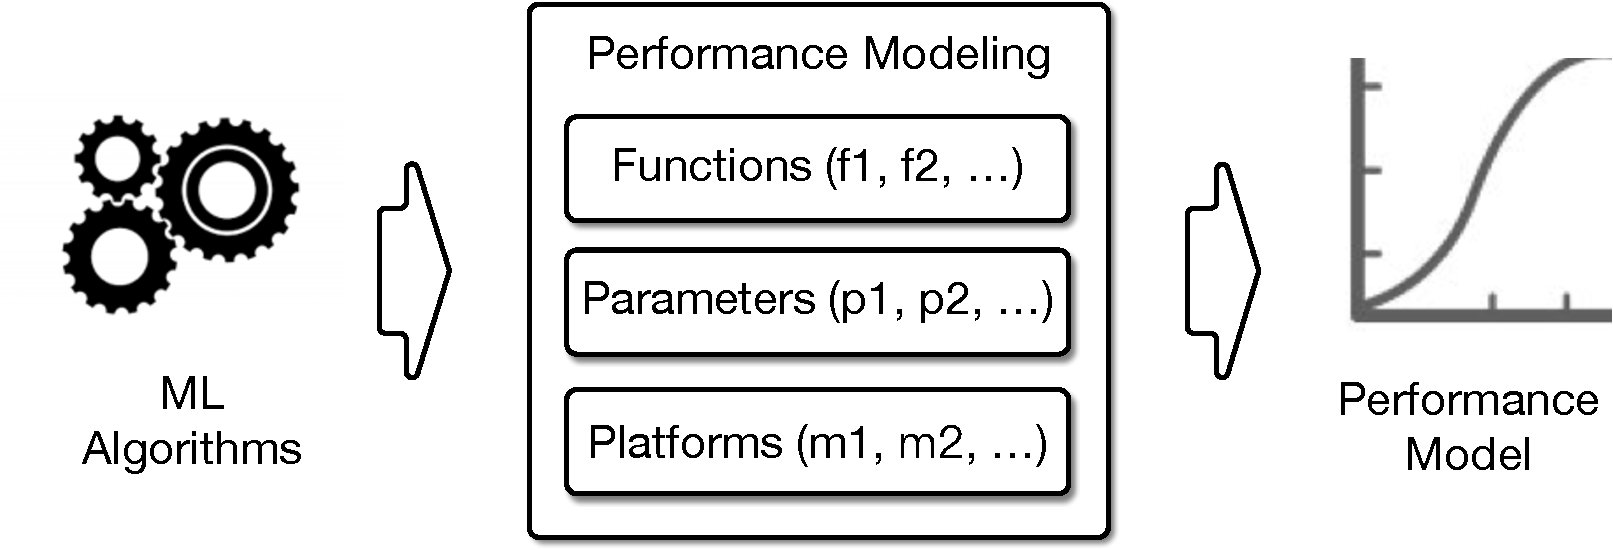
\includegraphics[width=0.9\columnwidth]{figures/offline.pdf}
    \caption{Performance modeling.}
  \end{subfigure}
  \\
  \vspace{1em}
  \begin{subfigure}[t]{0.8\columnwidth}
    \centering
    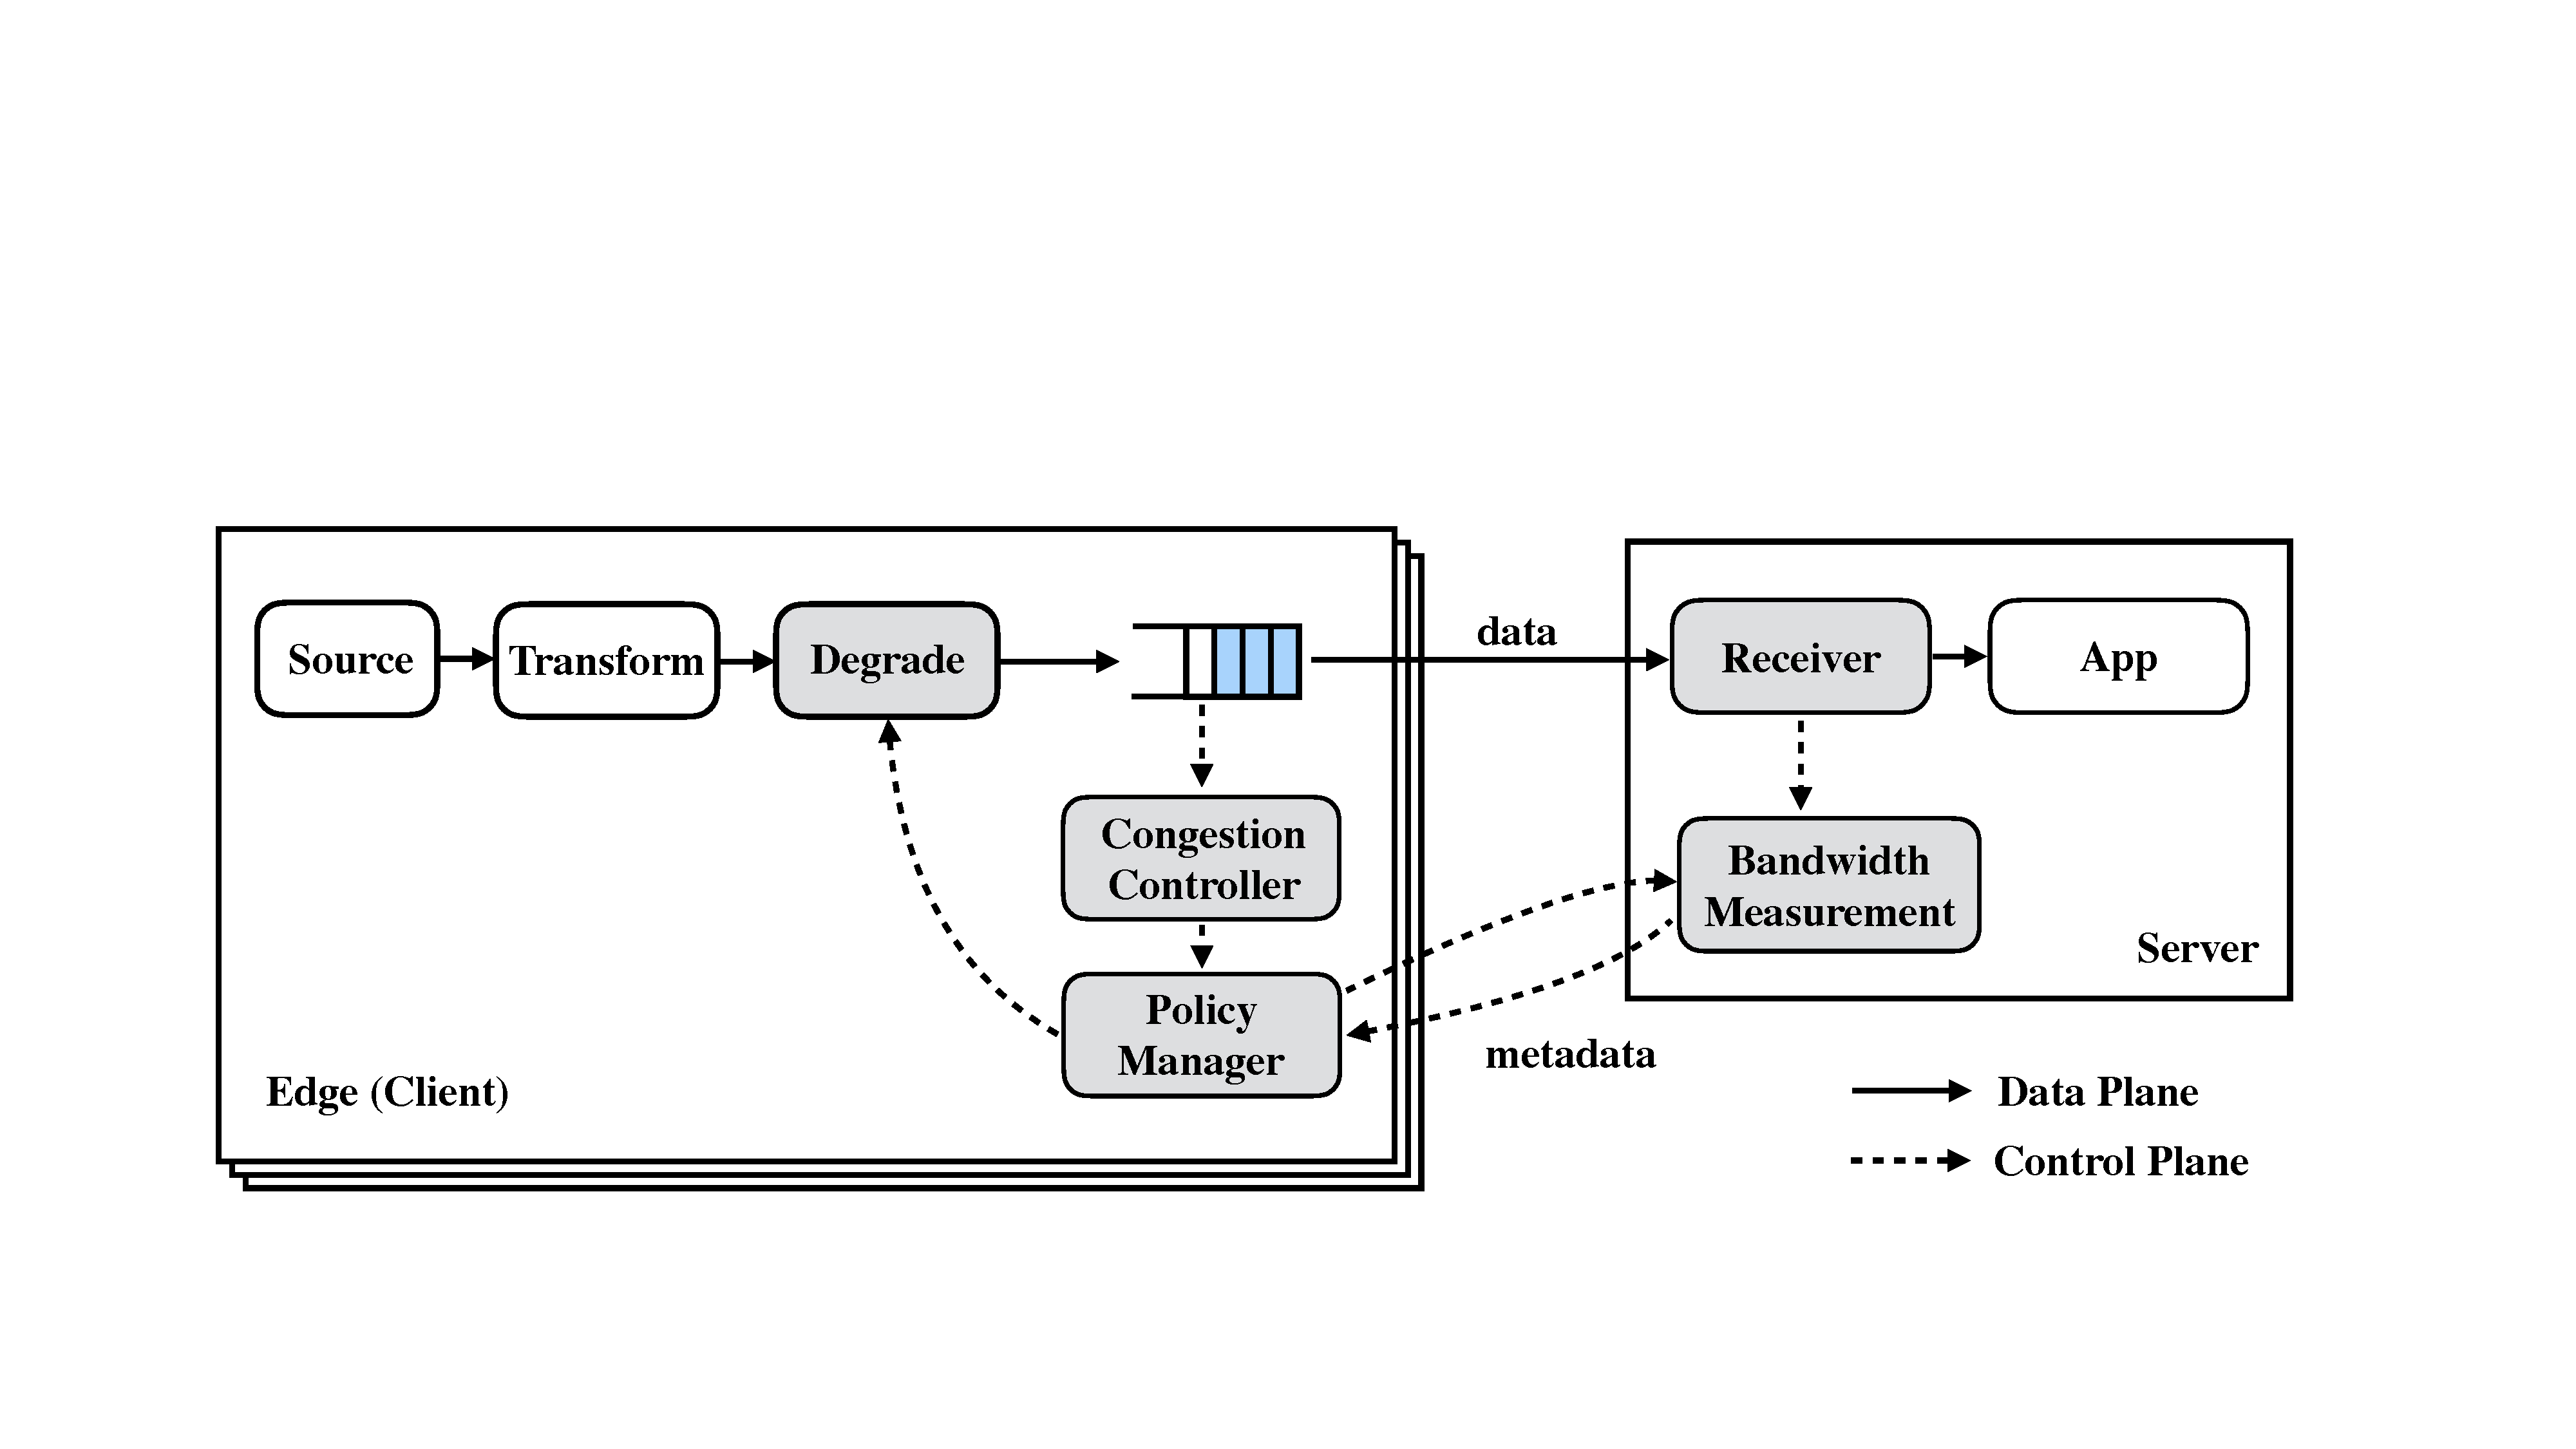
\includegraphics[width=\columnwidth]{figures/runtime.pdf}
    \caption{Runtime dispatch and service triage.}
  \end{subfigure}%
  \caption{\sysname{} Architecture.}
  \label{fig:system}
\end{figure}

We design \sysname{} to address the aforementioned challenges. The architecture
involves two part: performance modelling and runtime serving
(\autoref{fig:system}). \sysname{} integrates multi-objective optimization (MOO)
using Bayesian method to generate the Pareto-optimal set of configurations. To
transfer models across platforms, \sysname{} uses learned performance model as
\textit{a prior} and performs additional sampling if necessary. The client
dispatches requests using multi-armed bandit. The server performs continuous
triage and fast rejects if it cannot meet SLOs.

Before we dive into \sysname{}, we first present the application interface.

Developers don't need to care where exactly a particular function or service is
hosted, as long as it provides the desired output. We abstract the model serving
as a \texttt{predict} API similar to remote procedure call (RPC) interfaces.

\begin{lstlisting}
    predict(input: Input, p: SLA) -> Output
\end{lstlisting}

Internally, the return value is a tuple

\begin{lstlisting}
    Vec<(O: Output, t: Time, a:  Accuracy)>
\end{lstlisting}

\textbf{More to expand here.}

\textbf{How to configure trade-off.}

\section{Performance Modeling}
\label{sec:performance-modeling}

The first step towards bounded response times is to model the relationship
between accuracy and execution time. We then describe the formalism and our
data-driven approach.

\subsection{Problem Formulation}
\label{sec:problem-formulation}

We assume there are multiple algorithms $\mathbb{A}$ available to provide the
same inference. For each algorithm $a \in \mathbb{A}$, it has parameters tunable
to affect processing time $t$ and inference accuracy (or utility $u$). These
parameters could be related to data, such as lowering the image resolution, or
related to the algorithm, such as increasing the scaling factor in HOG. One
instance of the parameters forms a configuration
$\vec{c} = (k_1, k_2, \dots, k_n)$ with $n$ dimensions---we explicitly use the
arrow head here to emphasize configurations' high dimensionality. Running the
algorithm $a$ with a configuration $\vec{c}$ on a machine $m$ yields an
inference with utility $u$ and processing time $t$.

We denote this performance model as a mapping:

{\small \vspace{-1em}
  \begin{equation*}
f: (\mathbb{A} \times \mathbb{C} \times \mathbb{M}) \rightarrow
(\mathbb{R}\times \mathbb{R})
\end{equation*}
} where $\mathbb{A}$ is the set of all algorithms, $\mathbb{C}$ is the set of
all possible configurations, and $\mathbb{M}$ is the set of all machines. The
mapping returns two real values: execution time $t \in \mathbb{R}$ and utility
$u \in \mathbb{R}$. For convenience, we use $\vec{x}$ for the tuple $(a, c, m)$.
Also we use $f_t$ and $f_u$ for the mapping from variables to time $t$ and
utility $u$, respectively.

Bounding the response times is trivial if application accuracy can be
arbitrarily low. \sysname{} aims to minimize response times while maximizing
achievable accuracy---solving a multi-objective optimization problem,
specifically two objectives. For these problems in general, there is no single
optimal solution that jointly minimizes multiple objectives. Instead, there is a
collection of optimal solutions where for any solution, no objective can be
improved without damaging one of the other objectives. The goal of our
performance modeling is to derive such Pareto-optimal
set~\cite{collette2013multiobjective} across all possible
configurations. Formally, the Pareto-optimal set is defined as follows,

{\small \vspace{-1.2em}
  \begin{equation}
    \mathbb{P} = \{ \vec{x} \in \mathbb{X} : \{ \vec{x'} \in \mathbb{X}:
    f_t(\vec{x'}) < f_t(\vec{x}), f_u(\vec{x'}) > f_u(\vec{x}) \} = \varnothing\}
  \label{eq:pareto}
\end{equation}
\vspace{-1.2em}
}

\para{Challenge.} The Pareto-optimal set is easy if we know the mapping for all
possible arguments. However, in practice, the argument space is prohibitively
large, especially for configurations $\vec{c}$ that have many tunable
parameters. It is expensive to run all combinations. Besides, it is also
impossible because developers may not have target machines available.

\para{Solution Overview.} We tackle each dimension differently. For algorithms,
because their differences are substantial, our profiler evaluates all available
algorithms exhaustively. For each algorithm, to address the curse of
dimensionality of $\vec{c}$, we use BO to reduce space search and only find
near-optimal $c$s. For different machine $m$, because only $f_t$ depends on $p$,
we show that the Pareto-optimal set doesn't change if the execution time $f_t$
satisfies monotonicity. We approximate $f_t$ with a simple linear model.

\subsection{Composing Algorithms}
\label{sec:compose-models}

There are different algorithms. Different implementation for GPU and CPU.

We have to profile each individual algorithm.

Observation: their profile (the Pareto-optimal set) are composable by merge and
compare all of them.

\subsection{Modeling Parameters}
\label{sec:single-platform}

Evaluating all configurations across the large parameter space is prohibitively
expensive. To reduce the number of samples we need, \sysname{} builds a
performance model that is just accurate enough to allow us to distinguish
near-optimal configurations from the rest. This is similar to recent systems,
such as CherryPick~\cite{alipourfard2017cherrypick} and
BOAT~\cite{dalibard2017boat}, that use Bayesian optimization (BO) to improve
performance across a large number of configurations.

While previous approaches often transform the multi-objective problem into a
single-objective problem using scalarization techniques (an approach that is
expected to be suboptimal~\cite{knowles2006parego}.) We adopted the
PESMO~\cite{hernandez2016predictive}, which does not transform the
multi-objective problem into a single-objective. PESMO also has a low
computational cost. It grows linearly with respective to the total number of
objectives $K$.

\subsection{Modeling Machines}
\label{sec:performance-transfer}

We make the observation that $f_u(a, c, m)$ doesn't depend on $m$. If we assume
a monitonicity between $f_t(m_1)$ and $f_t(m_2)$, we can prove that the
Pareto-set is directly transferable. The monitonicity is a condition that if on
one platform it takes longer for one configuration,
i.e.\,$f_t(a, \vec{c}, m_1) < f_t(a, \vec{c'}, m_1)$, then it will take longer
on another platform, i.e.\,$f_t(a, \vec{c}, m_2) < f_t(a, \vec{c'}, m_2)$.

Based on these two assumption, one can prove that if $\vec{x}_i$ is in the
Pareto-optimal set $\mathbb{P}_1$ for platform $p_1$, then $\vec{x}_i$ will also
be in the Pareto-optimal set $\mathbb{P}_2$. And the profile on $p_2$ will be a
stretched or shrunk version for $p_1$ along the time dimension.

This simplifies our model transfer across platforms and makes it possible to
derive the performance model at runtime by sampling only a few performance
measures. In practice, a simple linear transformation suffices in giving a
reasonably precise transfer.

\section{Runtime System}
\label{sec:runtime-system}

\subsection{Client Dispatch}

The decision layer dispatches the requests to multiple instance of servers. The
decision is based on the service level aggreement (SLA) that developer
specficies. After servers complete the inference, results are returned and
merged. The merging process is similar to the \texttt{Reduce} phase in MapReduce
that combines the vector of return values into a single response. We provide a
few different merging policies corresponding to different SLAs:

\para{Earliest first}. For all running services, the earliest return will be
used first. When the user specifices SLA with minimal response time, policy
achieves the minimal possible response times.

\para{Eventual accurate}. For return type such as a set, the merge can be
automatically done by combining the individual results. In this way, the system
may return a less accurate result first for timeliness, but eventually, the
system will yield a higher accuracy. This requires either the return type
implements \texttt{Merge} interface. For common data types such as \texttt{Set}
or \texttt{List}, we've implemented the interface for developers. For advanced
types, as we will demonstrate in the image example, developers can implement
this interface by themselves.

\para{Bounded time}. With a configured time bound, \sysname{} will pick the
results with the highest accuracy that are within the deadline.

\para{Bounded accuracy}. With a configured lower bound on the accuracy,
\sysname{} will pick the results with the smallest response times.

At runtime, \sysname{} dispatches application request to multiple platforms and
combine their results transparently. It makes the decision of where to run (what
platform to use) and how to run (what configuration to use) to satisfy
application requirement. The decision is related with the desired guarantee the
developer has expressed using our API and the condition during the application
execution.

\para{Static scheduling.} Our baseline schedule makes decision based on an
estimation of the network latency and server response time. If the algorithm can
be executed locally, it will do. If the algorithm cannot run locally in full
accuracy, we shall do it locally, together with offloading requests to available
servers.

\para{Statistical scheduling.} We cast the dispatch as a multi-armed bandit
problem. Different from existing approaches where pulling each arm doesn't incur
much cost; in our settings, local processing and remote communication has an
associated cost. This is multi-armed bandit with budget.

\subsection{Server Calibration}

Calibrate the profile by running.

\subsection{Server Scheduling}
\label{sec:server-scheduling}

The server runs a novel real-time scheduling algorithm that maximizes the
throughput and achievable accuracy while meeting SLOs. \sysname{} employs a fast
reject if serving the new request will violate the SLOs of any pending
requests. By rejecting instead of queuing up, \sysname{} addresses server
contention and reduces tail latency even under contention.

Rejection must be a cheap operation to sustain large number of concurrent
requests. In \sysname{}, we maintain a variable \texttt{capacity} that is
updated whenever a worker thread starts or finishes serving. Determining
schedulability is essentially comparing the request's SLO with available
capacity.

\para{Scheduling}. Given each task with a deadline constrain and the degree of
freedom of trading off quality for processing times, the scheduler finds the
best scheduling strategy.

\para{Acceptance test}. Perform admission control at the arrival of requests to
verify the schedulability of the task set. If the task set is found schedulable,
the new task is accepted in the system; otherwise, it is rejected.

\para{Re-scheduling}. A naive scheduler will either always run at highest
quality with lowest throughput; or lowest quality with highest throughput. A
better scheduler that explores the trade-off but with a naive design will
perform re-scheduling at every job arrival. The desired scheduler only
re-schedules when necessary.

%%% Local Variables:
%%% mode: latex
%%% TeX-master: "../serving"
%%% End:

%% LocalWords: schedulability